\documentclass[10pt,a4paper]{beamer}
\usepackage[utf8]{inputenc}
\usepackage[francais]{babel}
\usepackage[T1]{fontenc}
\usepackage{amsmath}
\usepackage{amsfonts}
\usepackage{amssymb}
\usepackage{makeidx}
\usepackage{graphicx}
\usepackage{datetime}
\usepackage{color}
\mode<presentation>

\usetheme{Warsaw}
\newdate{date}{11}{06}{2014}

\definecolor{monRouge}{RGB}{204,0,0}
\setbeamercolor{block body alerted}{fg=white,bg=monRouge}

\author{Frémont Alexandre et Le Calvar Théo}
\title{probleme des n-dames}
\date{\displaydate{date}}
%\institute{\includegraphics[width=0.3\textwidth]{images/ua_h_couleur.jpg}}

\begin{document}

\begin{frame}
\titlepage
\end{frame}

\begin{frame}
	\frametitle{Plan}
	\tableofcontents[pausesections]

\end{frame}

\section{Introduction}
\begin{frame}

	\begin{block}{Introduction}
	Le problème des N-Dames est une extension du problème des 8 dames, son
	but est de placer 8 dames d’un jeu d’échecs sur un échiquier de façon à ce
	qu’aucune ne soit menacée.

	\end{block}

\end{frame}

\section{structure de données}
\begin{frame}


	\begin{block}{Representation de l échiquier}
		\begin{itemize}
			\item{tabeau à une dimension}
			\item{tableau des domaines pour le foward checking}
			\item{tableau de diagonale pour la recherche local}
		\end{itemize}
	\end{block}


\end{frame}

\section{Algorithme}
\begin{frame}
	\frametitle{Algorithme}

	\begin{block}{Backtracking}
		On construit l'échiquier par étape, lorsque une iteration viole une contrainte on retourne en arrière et on change l'itération.
	\end{block}



	\begin{block}{Forward checking}
		On place nos dames sur l'échiquier et à chaque dame placé on diminue l'espace ou l'on poura placé nos futurs dames \\
		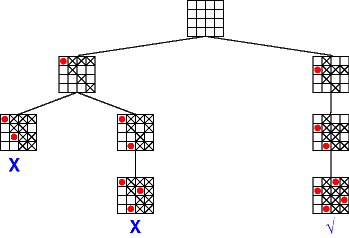
\includegraphics[width=0.4\textwidth]{images/forw.png}
	\end{block}

\end{frame}


\section{Algorithme de recherche local}
\begin{frame}
	\frametitle{Algorithme}

	\begin{block}{1er algorithme de recherche local}
		\begin{itemize}
			\item{initialisation}
			\item{transposition entre les dames}
			\item{descente stricte}
		\end{itemize}
	\end{block}

	\begin{block}{2nd algorithme de recherche local}
		\begin{itemize}
		      \item{initialisation a 100 conflits}
		      \item{transposition entre les dames}
		      \item{descente stricte}
		      \item{reset si bloqué}
	      \end{itemize}
	\end{block}


\end{frame}

\section{Resultat et performance}
\begin{frame}
	\frametitle{Resultat et performance}

	\begin{block}{Backtrack}

	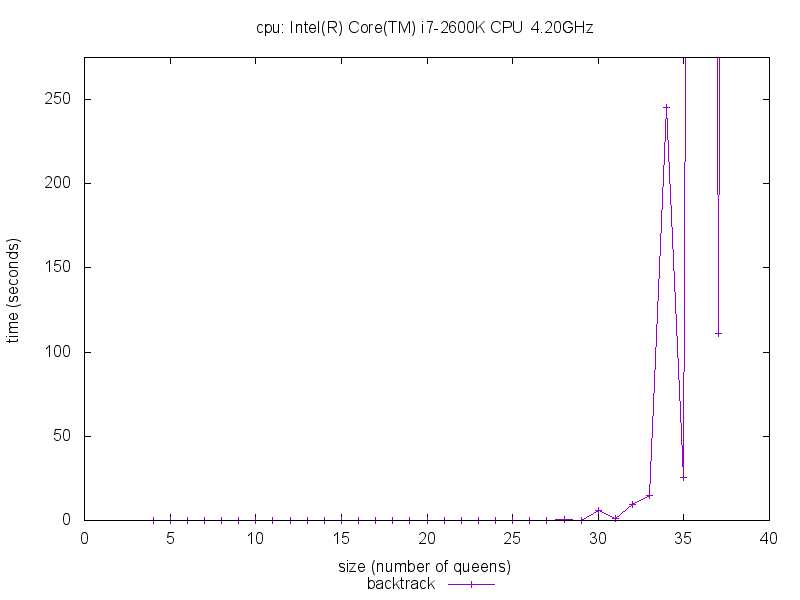
\includegraphics[width=0.3\textwidth]{images/plot_bt_i7.png}

	\end{block}

	\begin{block}{Forward}

	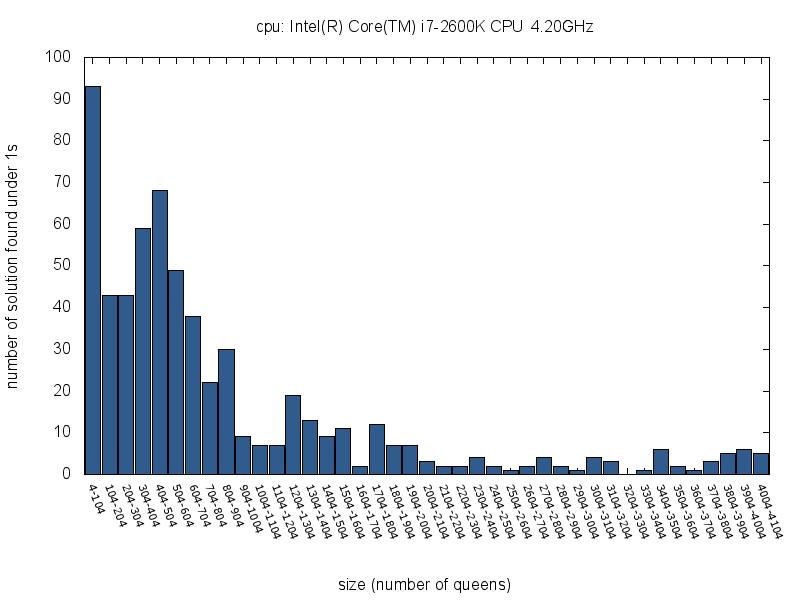
\includegraphics[width=0.3\textwidth]{images/plot_fw_i7.png}

	\end{block}

	\begin{block}{backtrack vs Forward}

	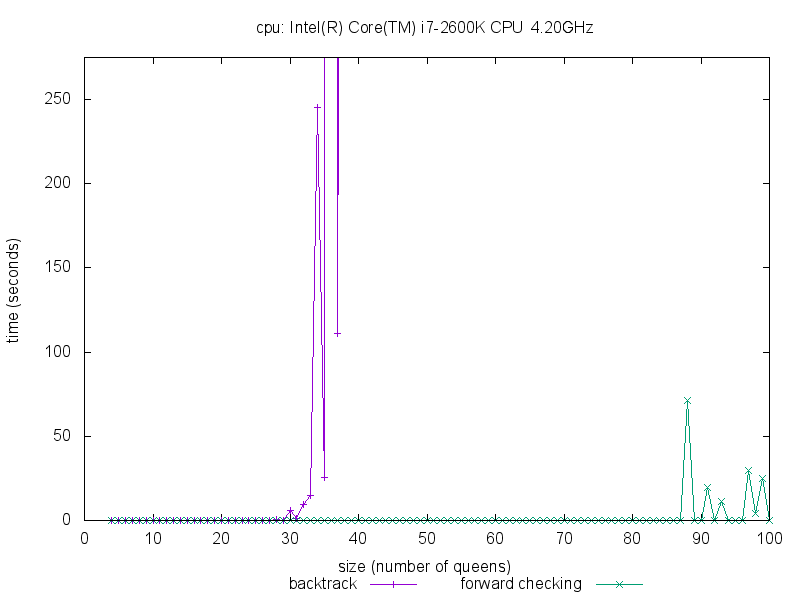
\includegraphics[width=0.3\textwidth]{images/plot_bt_fw_i7.png}

	\end{block}



\end{frame}

\section{Resultat et performance}
\begin{frame}
	\frametitle{Resultat et performance}

	\begin{block}{recherche local}

	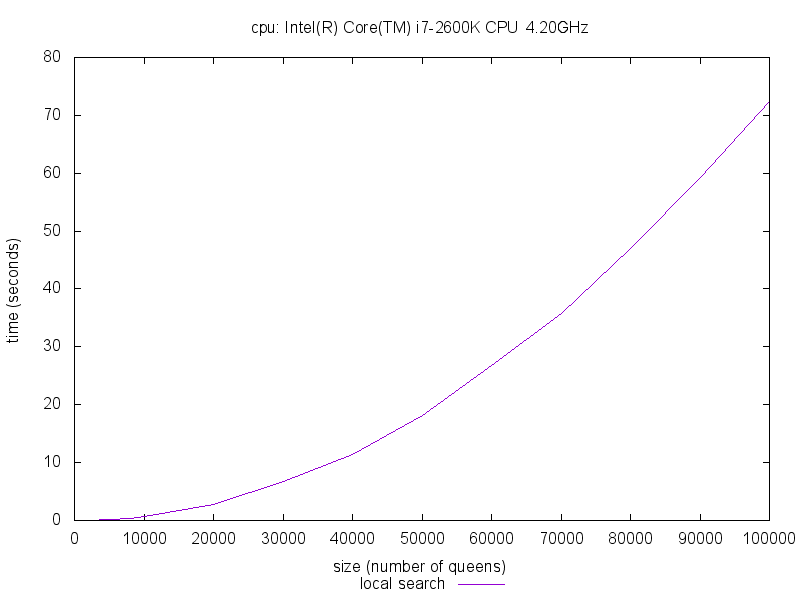
\includegraphics[width=0.3\textwidth]{images/plot_ls_i7.png}

	\end{block}

	\begin{block}{recherche local amélioré}

	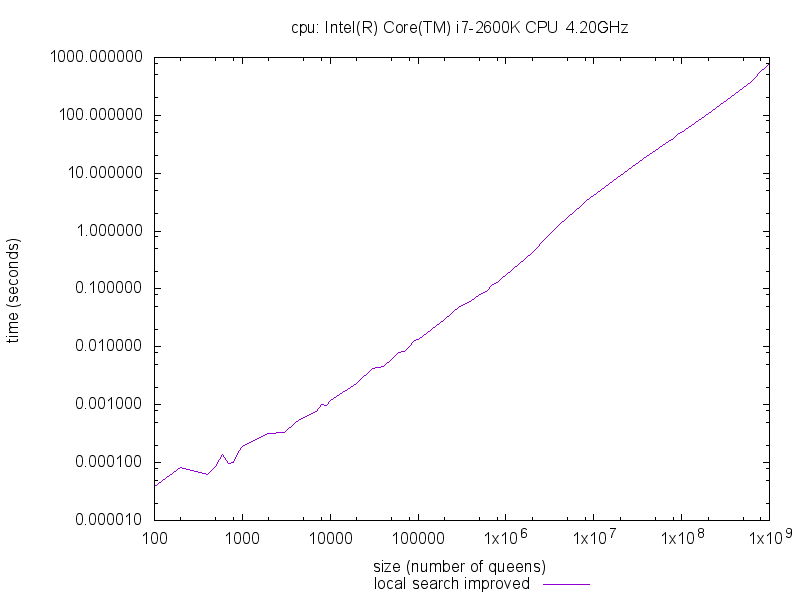
\includegraphics[width=0.3\textwidth]{images/plot_lst_i7.png}

	\end{block}

	\begin{block}{comparaison}

	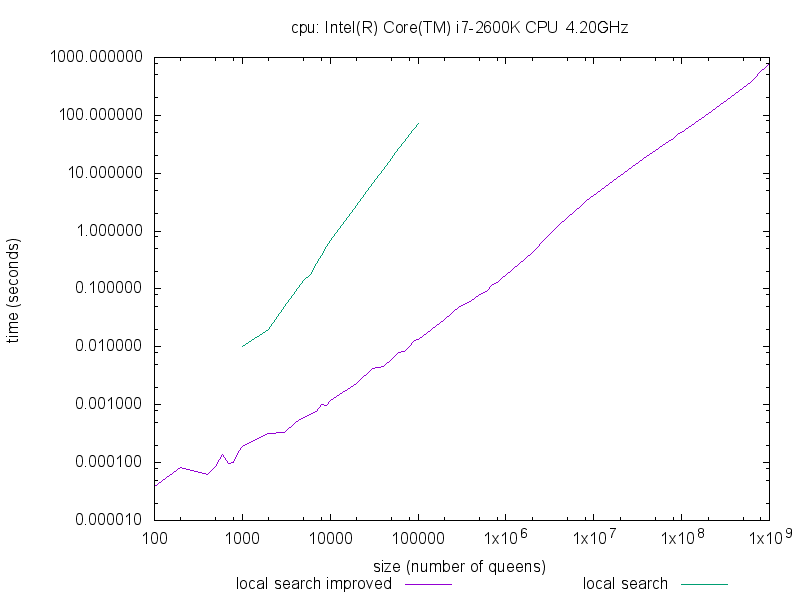
\includegraphics[width=0.3\textwidth]{images/plot_lst_ls_i7.png}

	\end{block}



\end{frame}

\section{Conclusion}
\begin{frame}
	\frametitle{Conclusion}

	\begin{block}{avantage et inconvenient}
	      \begin{itemize}
		      \item{backtrack et forward checking certitude de l'obtention d'un résultat}
		      \item{mais au bout de combien de temps}
		      \item{methode de recheche local pas sur d'aboutir}
		      \item{mais s'effectue très rapidement}
	      \end{itemize}
		
	\end{block}


\end{frame}


\end{document}
